\chapter{Dynamic Models: Part 1}\label{c:model1}
\renewcommand{\epigraphsize}{\small\itshape}
\renewcommand{\epigraphwidth}{4.25in}
\renewcommand{\epigraphrule}{0pt}
\begin{epigraphs}
\qitem{The best material model of a cat is another, or preferably the same cat.}{--- \textup{Arturo Rosenblueth and Norbert Wiener}, \\The Role of Models in Science, 1945.}
\end{epigraphs}

\section{All Models Are Wrong!}
For our purposes a \emph{model} is equivalent to a \gls{mathematical model}, an equation.  We can use to understand and design a \emph{system}, a physical system which we wish to analyze.  Over the last few hundred years people with last names like Newton, Maxwell, Euler, Lagrange  and Bernoulli have come with with a variety of simple equations that describe physical processes.  The key point, that is often overlooked, is that this description is only approximate; the mathematical model and the physical system never share the same behavior.

So why do engineers spend so much time and energy learning mathematical equations and how to solve them if these models never completely capture the behavior of a physical system?  It turns out that under specific conditions, these models allow us to \emph{predict} the behavior of systems that we might want to build.  

As an example, consider the Hoover Dam, a \unit[726]{ft} tall structure constructed with over 3 million cubic yards of cement.  In designing this structure we would hope that engineers spent a large amount of time on structural models to attempt to predict if their designs would last through floods, earthquakes and any situation that might arrive.  Without any models they would be have to fall back on the build-and-test process of engineering, building a prototype dam and sitting back to see if it worked; obviously not a very safe or cost effect way to build a dam.  On the other hand, we have to imagine that the engineers included some conservative factors of safety to build the structure somewhat larger and stronger than their models predicted.  They did this because they understood that the model was only an approximation of the dam; the model was wrong, but still useful.  

So, even though models are wrong (they are always simplified approximations), they are useful for the following reasons:
\begin{itemize}
\item under certain specific conditions mathematical models can predict (approximately) the behavior of physical systems
\item analysis of the model behavior can be an efficient way to test the behavior of system designs before we go to the trouble (cost and time) to build the physical system
\item we can analyze the behavior of models in situations that would be hard or impossible to create in the physical system
\item the model analysis enables us to understand the system and build intuition about how a system behaves 
\end{itemize}

\section{First-Order Model}
Our \gls{first-order model}, a first-order, linear, ordinary differential equation, is 
\begin{equation}
\label{e:first}
\frac{dy(t)}{dt} + \frac{1}{\tau}y(t) = f(t).
\end{equation}
where $f(t)$ is the input (forcing function), $y(t)$ is the output (response function) and $\tau$ is the time constant.  That's it; there is really nothing more to say.  

But of course we do have much more to say.  I want to start by emphasizing that this model is just as wrong as the rest of them (but it can be very useful).  There are two reasons that this model is useful:
\begin{enumerate}
\item The time-response of this model is sufficiently similar to that of many physical systems to allow us to use this fictitious model (equation) to predict how an actual system might behave.
\item We know (or we will know shortly) how to solve this equation to calculate the output of the model in response to a variety of inputs.
\end{enumerate}

\subsection{An Example}
One example of a physical system that can be approximated by our first-order model is a automobile.  Let's consider how the speed of an automobile (the output) responds to changes in the gas petal (the input) as it moves in a constant direction.  The sketch if Figure~\ref{f:massd} illustrates this simplification of a complex physical system. 
\begin{figure}[hbt!]
\centering
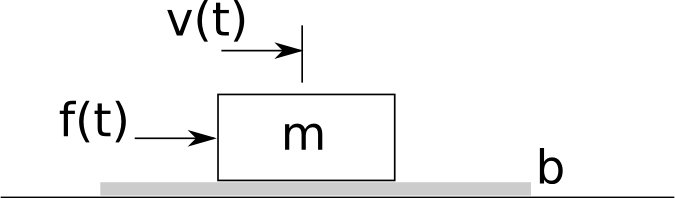
\includegraphics[width=\FigWidth\textwidth]{mass_damper.png}
\caption{Sketch of a simplified automobile model.  The point mass ($m$) moves to the right at a velocity ($v(t)$.  The input is a force ($f(t)$).  There is a drag force that resists the motion. }
\label{f:massd}
\end{figure}
Based on this sketch we can do things like draw a free-body-diagram and apply Newtonian principles to arrive at an equation of motion.  We might also make an ambitious simplifying assumption that the drag force that resists the motion of the mass is linearly related to the velocity, i.e., $f_{\mathrm{drag}}=b(v(t))$.  We could come up with an equation of motion, our mathematical model,
\begin{equation}
\label{e:car}
m\left(\dot{v}(t)\right) + b(v(t)) = f(t)
\end{equation}
where $m$ is the mass of the car, $v(t)$ is the speed, $\dot{v}(t)$ is the acceleration, $b$ is the coefficient of linear drag and $f(t)$ is the input force.
This equation has the same form (a first-order, linear, ordinary differential equation) as our first-order model~(\ref{e:first}).

This is meant to be an example of a model that is obviously wrong.  A physical automobile is a complex system with many, many degrees of freedom.  Our simplified model~(\ref{e:car}) is meant to do just one thing, allow us to predict how, in general, the speed of a car responds to changes in the throttle input.

\section{Step Response}\label{s:firststep}
One useful aspect of our first-order model~(\ref{e:first}) is that the solution to this differential equation is well known for a variety of input functions.  A particularly interesting input function is the \gls{step function} ($\mu(t)$) defined as
\begin{equation}
\label{e:step}
\mu(t)= \left\{ 
\begin{array}{cl}
0 & \, \mathrm{for}\, t < 0 \,\,\,\\
1 & \, \mathrm{for}\, t \geq 0
\end{array} \right.
.
\end{equation}
Figure~\ref{f:step} illustrates how the value of $\mu(t)$ is zero before $t=0$ and then instantaneously changes to unity.
\begin{figure}[hbt!]
\centering
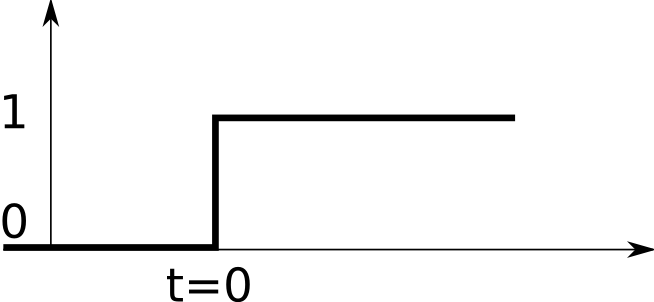
\includegraphics[width=\FigWidth\textwidth]{step.png}
\caption{Illustration of a step function $\mu(t)$.}
\label{f:step}
\end{figure}

The \gls{step response} of our first-order model is the solution to (\ref{e:first}) with step function as the input ($f(t)=A\mu(t)$) and an initial condition of zero ($y(0)=0$).  (You should notice that the step function here has an amplitude of $A$ rather than an amplitude of 1 as indicated in (\ref{e:step}).)  The step response is the well known solution
\begin{equation}\label{e:stepresp}
y(t) = A\tau\left(1-e^{-t/\tau}\right)
\end{equation}
for $t>0$.

\begin{figure}[hbt]
\centering
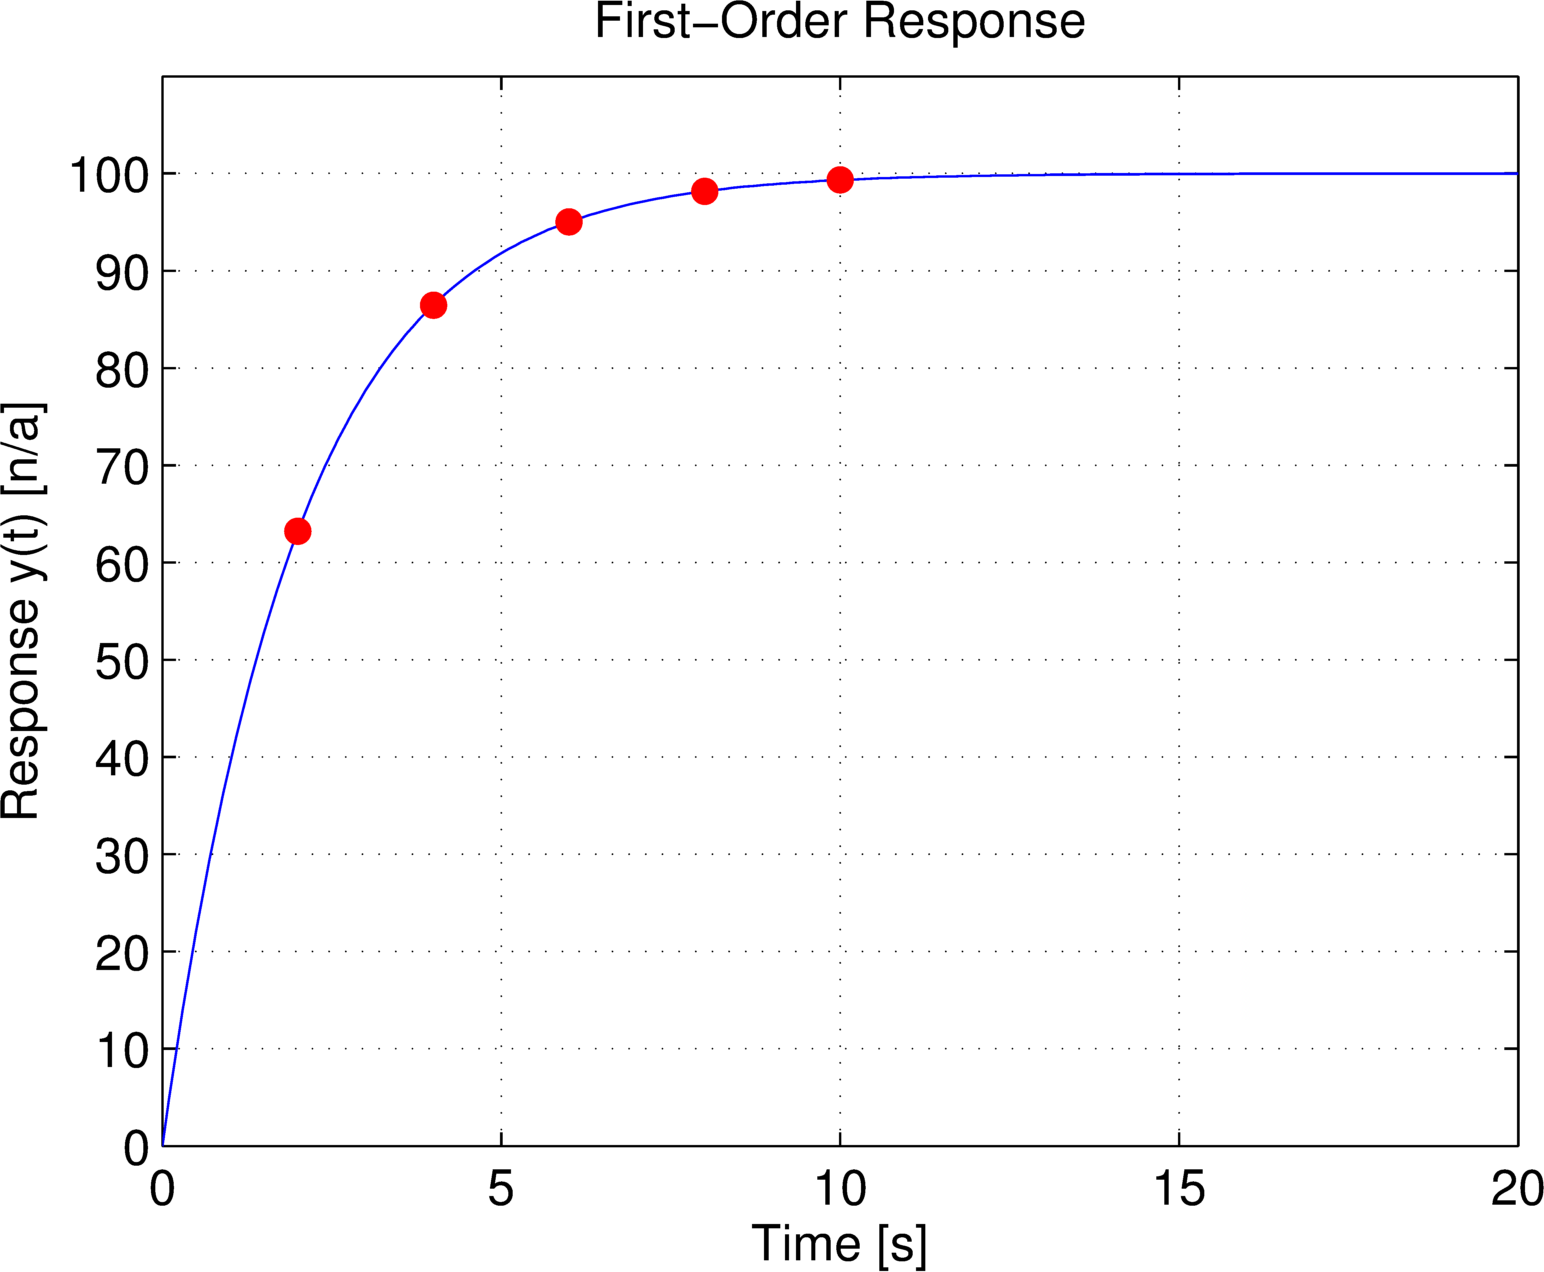
\includegraphics[width=\textwidth]{first_step.png}
\caption{Graph of the step response (\ref{e:stepresp}) with $\tau=\unit[2]{s}$ and $A=50$.  The red dot markers indicate the value of the solution at $t=[\tau,2\tau,3\tau,4\tau,5\tau]$. }
\label{f:firststep}
\end{figure}


\lstinputlisting[style=myMatStyle,
caption={code},
label={l:firstresp}]
{./code/first_order_response.m}


This solution is graphed in Figure~\ref{f:firststep} using the MATLAB script in Listing~\ref{l:stepresp}. This time response to a step input (or step response for short) has a characteristic shape as it rises and approaches the \gls{steady-state response} exponentially.  One important aspect of the response is that it approaches a new constant value, the steady-state response.  A simple way to find the steady state value is to set $\dot{y}(t)=0$ in (\ref{e:first}).  Since we are looking for the ``steady-state'' value we can anticipate that all rates of change (derivatives) will be zero.  Now the steady-state value ($y_{\mathrm{ss}}$) is 
\begin{equation}\label{e:ss}
y_{\mathrm{ss}} = \tau A
\end{equation}

Another important characteristic of this model is that the response ($y(t)$) moves exponentially from the initial value to the steady state value.  This response is characterized by the the \gls{time constant} ($\tau$).  If we evaluate time response (\ref{e:stepresp}) at $t=\tau$ we find that
\[
y(t=\tau) = A \tau (0.632) = 0.632 (y_{\mathrm{ss}})
\]
which means that after one time constant has passed the response is 63.2\% of the way from the initial value to the steady state value.  Take a look at Figure~\ref{f:firststep} to make sure that we did the math correctly!

\subsection{An Example}
Now that we've discussed the time response of our first-order model let's see how this applies to our automobile model.  We can rearrange the mathematical model (\ref{e:car}) so that it looks more like our generic model (\ref{e:first})
\begin{equation}\label{e:car2}
\dot{v}(t) + \frac{1}{m/b}(v(t)) = \frac{F}{m}\mu(t))
\end{equation}
which highlights that the time constant is $\tau=m/b$ and that the steady state speed is $v_{\mathrm{ss}}=F/b$.  Take a moment to think about this.  It means that the larger the mass of our car, the slower the acceleration (because the time constant is larger).  You might also notice that the mass has no effect on the steady state speed; our model says that a heavy ``car'' will reach the same final speed as a light car, it will just get there slower.  Finally we might notice that the more drag in our model, the slower our ``car'' will go for the same input.   

\begin{ex}
The step function in (\ref{e:step}) could be more precisely called the ``unit step function'' because it has an amplitude of 1.  Write an equation (similar to (\ref{e:step})) and sketch a graph (similar to Figure~\ref{f:step}) for the more general step function input $f(t) = A(\mu(t-t_o))$.
\end{ex}

\begin{ex}
We justified (\ref{e:ss}) by starting with the model (\ref{e:first}).  Another way to calculate the steady state response is to evaluate the solution (\ref{e:stepresp}) as $t \to \infty$.  Show that using this method yields the same result.
\end{ex}

\begin{ex}
We showed that the response of a first-order model to a step function input has an exponential increase characterized by the time constant.  Furthermore we showed that after a duration of one time constant beyond the rise in the step input the output will be 63.2\% of the way to its steady state value.  Figure~\ref{f:firststep} illustrates the value of the response at  $t=[\tau,2\tau,3\tau,4\tau,5\tau]$.  Evaluate \ref{e:stepresp} for these values of time and report the results in a two column table where the first column is the ratio $t/\tau$ and the second column is the ratio $y(t)/y_{\mathrm{ss}}$.
\end{ex}

\begin{ex}
Consider the step response to our car model (\ref{e:car2}) with the following parameters: mass = \unit[750]{kg}, drag coefficient = \unitfrac[150]{Ns}{m}, step input amplitude = \unit[10,000]{N}.  Create a graph similar to Figure~\ref{f:firststep} to illustrate the step response of our ``car''.  Annotate the graph to show the time constant and the steady state speed.  Also, make sure to use appropriate units for each axis.
\end{ex}

\begin{ex}
Consider the step response to our car model (\ref{e:car2}) with the following parameters: mass = \unit[750]{kg}, drag coefficient = \unitfrac[150]{m}{s}.
\begin{itemize}
\item What is the minimum step input amplitude ($F_{\mathrm{min}}$ that would cause our ``car'' to go from \unit[0--60]{mph}?
\item Based on this minimum step input amplitude, how long does it take for the ``car'' to go from \unit[0--60]{mph}?
\item If we double ($F_{\mathrm{min}}$
 \begin{itemize}
 \item How long does it take for the ``car'' to go from \unit[0--60]{mph}?
 \item What is the new top speed (in mph)?
 \item How long does it take for the ``car'' to achieve this new top speed?
 \end{itemize}
\end{itemize}
\end{ex}

\section{Free Response}
Another useful time response of our first-order model is the response with no input ($f(t)=0$) and an initial condition ($y(0)=y_o$).  The solution to (\ref{e:first}) under these conditions is 
\begin{equation}\label{e:firstfree}
y(t) = y_o \, e^{-t/\tau}
\end{equation}
for $t>0$. Figure~\ref{f:firstfree} illustrates this free response.  Just as before the time constant is the key factor that determines the characteristic of the response.  Again, at $t=\tau$ the output has fallen by 63.2\%.
\begin{figure}[hbt]
\centering
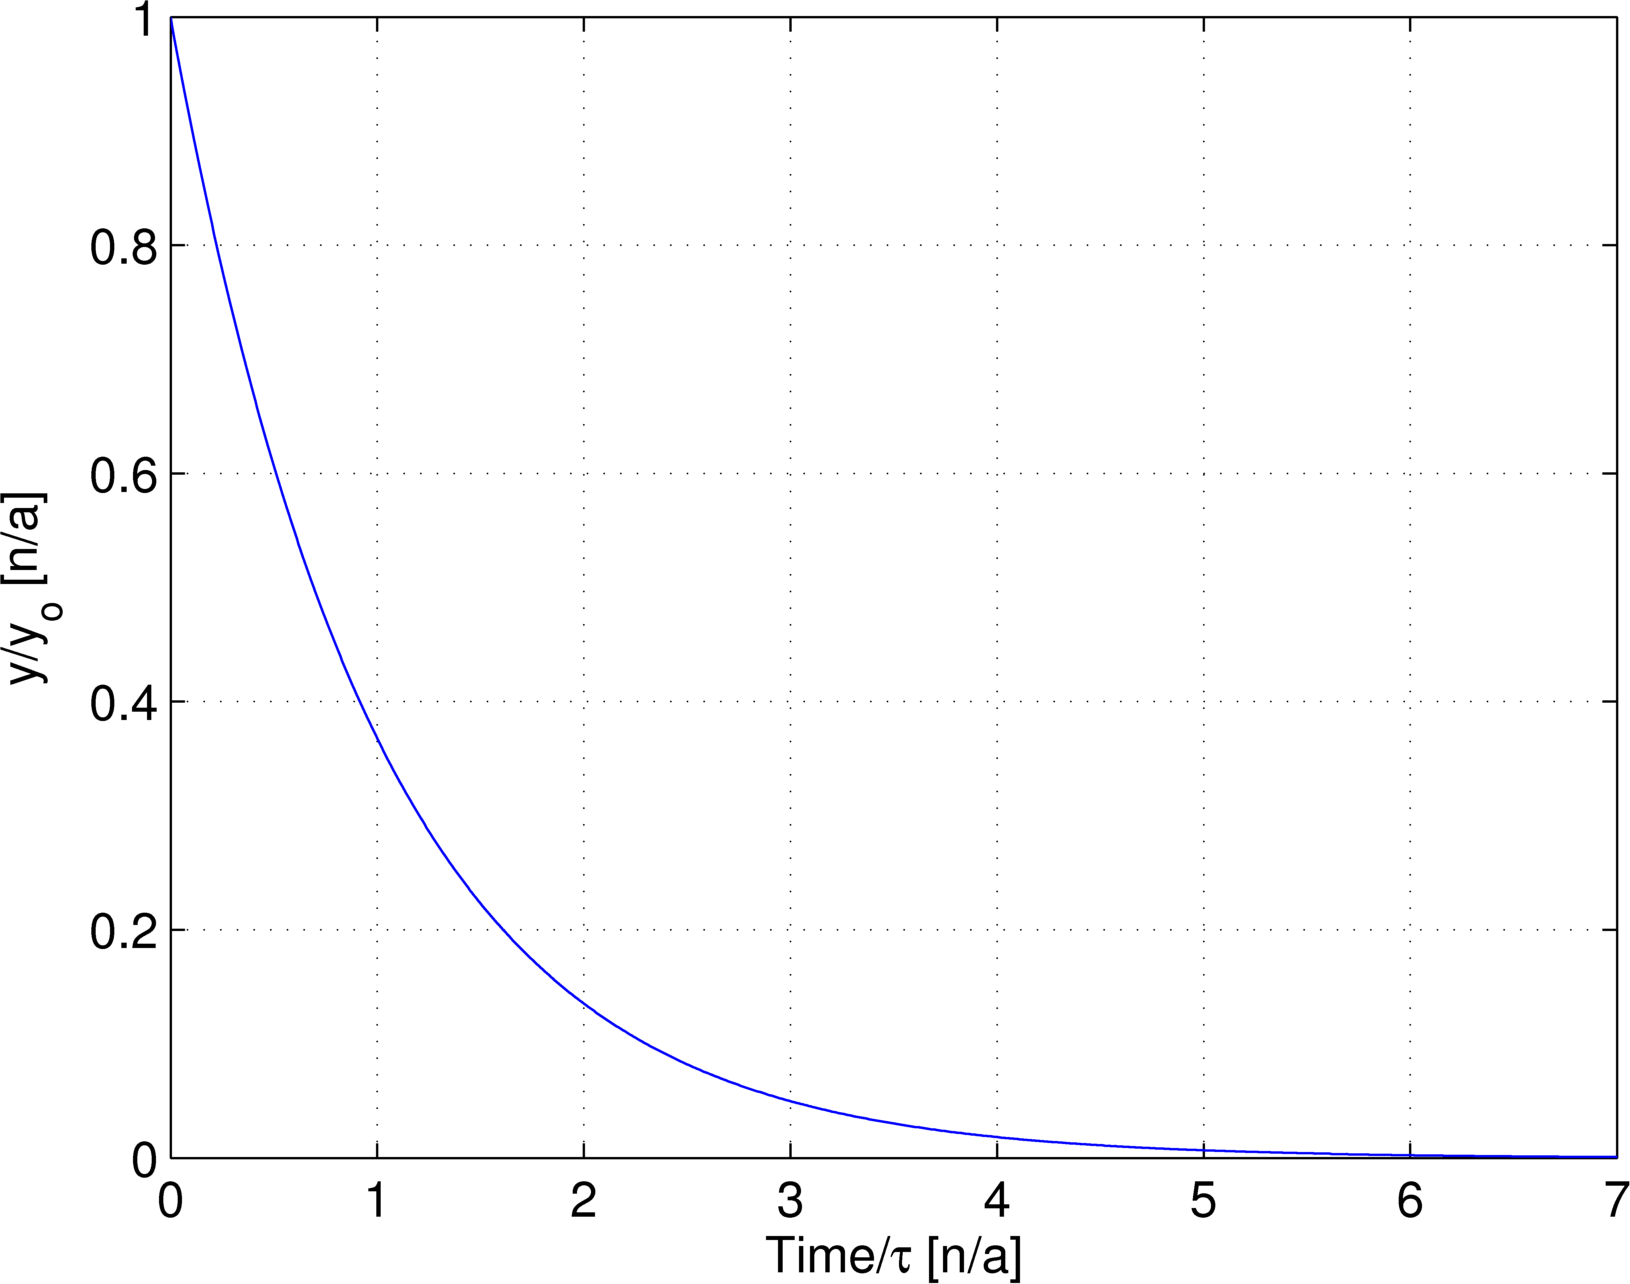
\includegraphics[width=\FigWidth\textwidth]{firstfree.png}
\caption{Graph of the free response (\ref{e:firstfree}).  Notice that the $x$ and $y$ axes have been normalized so that the output is the ratio of the response and the initial condition and the time is the ratio of time and the time constant.}
\label{f:firstfree}
\end{figure}

\begin{ex}
Using our automobile model (\ref{e:car}), write an expression for the free response of this model with appropriate physical parameters.  Create a graph of the free response with the initial condition $v(0)=\unit[60]{mph}$. For the x-axis of the graph use the units mph and for the y-axis of the graph use the units seconds.
\end{ex}

\section{Superposition}
One the characteristics that make linear system such as our first-order model useful is the principle of \gls{superposition} which allows determine the solution to a linear model by adding together multiple solutions.  As an example, suppose there are two input functions, $f_1(t)$ and $f_2(t)$, and that the corresponding solutions are $y_1(t)$ and $y_2(t)$.  If we want to know the response of the system to both inputs, $f(t)=f_1(t)+f_2(t)$, we can simply add the two solutions, $y(t)=y_1(t)+y_2(t)$. 

This principle simplifies the task of finding the response to our first-order model when there are both initial conditions and a forcing function.  Armed with this we can determine the step response of our first-order model when there is a non-zero initial condition
\begin{equation}
y(t) = y_o \, e^{-t/\tau} + A\tau\left(1-e^{-t/\tau}\right)
\end{equation}

Another handy aspect of superposition is the scaling property.  This means that if we scale (multiply) the input by a factor ($a$) then the output is simply the response to the original input scaled (multiplied) by the same factor.  As an example, consider our first-order car model (\ref{e:car}) where the input is a force ($f(t)$).  If we know that a force of \unit[1,000]{N} results in a steady state speed of \unit[25]{mph} then superposition tells us that a force of \unit[2,000]{N} will result in a final speed of \unit[50]{mph}.

\begin{ex}
Consider our first-order car model discussed above where a \unit[1,000]{N} input yields a steady state speed of \unit[25]{mph}.  Furthermore, we know that the time constant of this system is \unit[2]{s}.  Again we double the input to \unit[2,000]{N}. What is the time constant with the doubled input?
\end{ex}

\section{Thermometer Example}
Our first-order model can be used to describe the response of a temperature sensor to changes in the ambient environment.  This is analogous to our ``car'' model in that the temperature sensor has thermal inertia (analogous to the mass of our ``car'') and thermal resistance (analogous to the drag of our ``car'').  

\subsection{Mathematical Model}
Suppose we have a bulb thermometer that is at equilibrium the instant before it is plunged into boiling water.  The measured temperature will not instantly move to \unit[100]{$^{\circ}$C}, but instead the temperature of the device ($T(t)$) will move toward the new equilibrium over time.  The speed of that response is determined by the inertia and resistance of the system.

Figure~\ref{f:therm} illustrates how we might analyze this system.  Newton's law of cooling says that ``the rate of heat loss of a body is proportional to the difference in temperatures between the body and the surroundings'', or, stated mathematically 
\begin{equation}
\dot{Q}=hA (T_f-T(t))
\end{equation}
where $\dot{Q}$ is the rate of heat transfer, $h$ is the heat transfer coefficient, $A$ is the surface area of the thermometer, $T_f$ is temperature of the surroundings and $T(t)$ is the temperature of the thermometer.  Furthermore the thermal energy in the thermometer mass is $Q=C(T(t))$ where $C$ is the total heat capacity (the product of the mass ($m$) and the specific heat capacity of the material ($c_p$)).  Putting this together we can come up with a first-order model for a thermometer
\begin{equation}
\label{e:therm}
\dot{T}(t)= \frac{hA}{C}(T_f-T(t)).
\end{equation}

\begin{figure}[hbt]
\centering
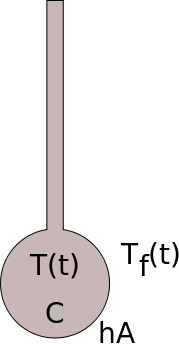
\includegraphics[width=0.20\textwidth]{thermometer.png}
\caption{Illustration of a simple model of the response of a thermometer.}
\label{f:therm}
\end{figure}

\begin{ex}
Using (\ref{e:therm}) rearrange the terms so that the expression has the same form as our canonical first-order model (\ref{e:first}).    What is the input to our model?  What is the output of our model?  What is the time constant of this model?  What is the steady-state temperature predicted by this model?
\end{ex}

